\documentclass[unicode,12pt,aspectratio=169]{beamer}

\graphicspath{{../fig/}}
%%%%%%%%%%%%%%%%%%%%%%%%%%%
\usepackage{luatexja}% 日本語したい
\usepackage[haranoaji,no-math,deluxe,expert,nfssonly,match,scale=1.0]{luatexja-preset}
\renewcommand{\kanjifamilydefault}{\gtdefault}% 既定をゴシック体に

\usepackage{amssymb,amsmath,ascmac}

\usepackage{multirow}
\usepackage{lltjext}

\usepackage{siunitx}
\usepackage{physics}
\AtBeginDocument{\RenewCommandCopy\qty\SI}
\ExplSyntaxOn
\msg_redirect_name:nnn { siunitx } { physics-pkg } { none }
\ExplSyntaxOff

\usepackage{animate}
\usepackage{svg}
\usepackage{xparse}
%%%%%%%%%%%%%%%%%%%%%%%
\usepackage{tikz}
\usetikzlibrary{shapes,arrows}
\usetikzlibrary{positioning}
\usetikzlibrary{angles,quotes}
\usetikzlibrary{math, calc}
\usetikzlibrary{decorations.markings,decorations.pathmorphing}
%% define fancy arrow. \tikzfancyarrow[<option>]{<text>}. ex: \tikzfancyarrow[fill=red!5]{hoge}
\tikzset{arrowstyle/.style n args={2}{inner ysep=0.1ex, inner xsep=0.5em, minimum height=2em, draw=#2, fill=black!20, font=\sffamily\bfseries, single arrow, single arrow head extend=0.4em, #1,}}
\NewDocumentCommand{\tikzfancyarrow}{O{fill=black!20} O{none}  m}{
\tikz[baseline=-0.5ex]\node [arrowstyle={#1}{#2}] {#3 \mathstrut};}

%目次スライド
% \AtBeginSection[]{
%   \frame{\tableofcontents[currentsection]}
% }
%アペンディックスのページ番号除去
\newcommand{\backupbegin}{
\newcounter{framenumberappendix}
\setcounter{framenumberappendix}{\value{framenumber}}
}
\newcommand{\backupend}{
\addtocounter{framenumberappendix}{-\value{framenumber}}
\addtocounter{framenumber}{\value{framenumberappendix}} 
}

%%%%%%%%%%%  theme  %%%%%%%%%%%
% \usetheme{Copenhagen}
\usetheme{metropolis}
% \usetheme{CambridgeUS}
% \usetheme{Berlin}

%%%%%%%%%%%  inner theme  %%%%%%%%%%%
% \useinnertheme{default}

% %%%%%%%%%%%  outer theme  %%%%%%%%%%%
\useoutertheme{default}
% \useoutertheme{infolines}

%%%%%%%%%%%  color theme  %%%%%%%%%%%
%\usecolortheme{structure}

%%%%%%%%%%%  font theme  %%%%%%%%%%%
\usefonttheme{professionalfonts}
%\usefonttheme{default}

%%%%%%%%%%%  degree of transparency  %%%%%%%%%%%
%\setbeamercovered{transparent=30}

%%%%%%%%%%%  numbering  %%%%%%%%%%%
% \setbeamertemplate{numbered}
\setbeamertemplate{navigation symbols}{}
\setbeamertemplate{footline}[frame number]

%%%%%%%%%%%%%%%%%%%%%%%%%%%%%%%%%%%
% \setbeamertemplate{items}[default]
\setbeamertemplate{enumerate item}[default]

% セクション名だけをTOCに出力
\setcounter{tocdepth}{1}




\title{第3章 線形粘弾性理論とは？}
\date{\empty}

\begin{document}
\setbeamercolor{page number in head/foot}{fg=white}
\frame{\titlepage}
\begin{frame}{アウトライン}
    \tableofcontents
\end{frame}
\setcounter{framenumber}{0}
\setbeamercolor{page number in head/foot}{fg=black}

\section{線形応答について}
\subsection{関数について}
\begin{frame}
	\frametitle{関数について}
		% \Large
		まず、関数を直感的に理解することから始めましょう。
		\begin{block}{関数の直感的理解}
			\begin{itemize}
				\item 関数のイメージ
				\begin{itemize}
					% \Large
					\item ２つの変数 $x$ と $y$ があるとしたら、
					\item 入力を $x$ で表したときに、
					\item その出力 $y$ を決定する規則
				\end{itemize}
				% \Large
				\item 一般に、関数は
				\begin{itemize}
					\item 英語の function の頭文字を使って $f$ と表記。
					\item そのときに、入力の変数を明示的に $f(x)$ と表す。
				\end{itemize}
			\end{itemize}
		\end{block}
\end{frame}

\begin{frame}
	\frametitle{関数について}
		\centering
		\begin{minipage}{\textwidth}
			\begin{columns}[c, onlytextwidth]
			\column{.65\linewidth}
				\begin{block}{関数のイメージ}
					\begin{itemize}
						\item ある変数 $x$ に依存して決まる出力 $y$ を\\ 
						\textcolor{red}{決める方法（図の右上）}
						\item 入力 $x$ に対して出力 $y$ を与える\\
						\textcolor{red}{変換装置（図の右下）}
					\end{itemize}
				\end{block}
				
				\vspace{-3mm}
				\begin{block}{数式では}
					\begin{itemize}
						\item 入力 $x$ と出力 $y$ との関係を表現する数式
					\end{itemize}
				\vspace{-5mm}
				\begin{align*}
					y&=f(x) \\
					\text{出力}&=\text{関数} \left(\text{入力} \right)
				\end{align*}
				\end{block}
			\column{.35\linewidth}
				\vspace{-5mm}
				\begin{center}
					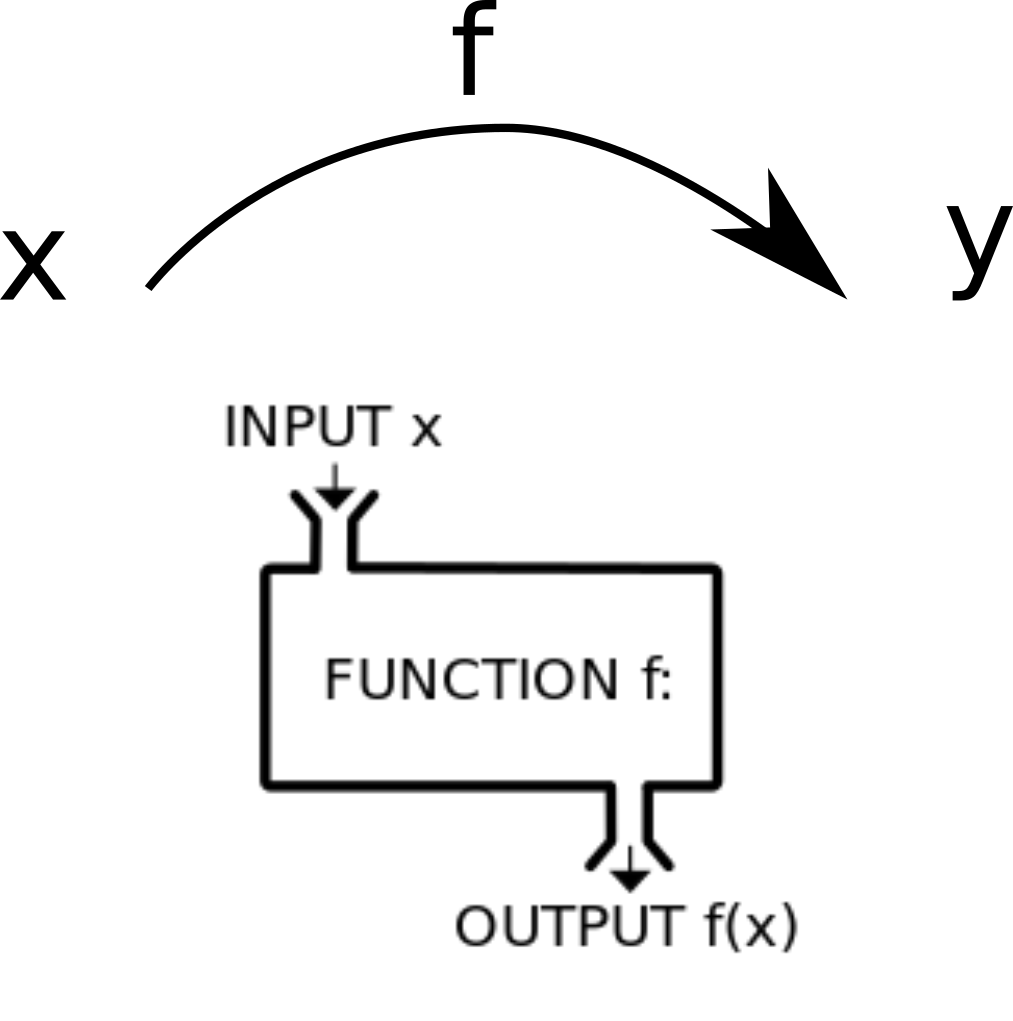
\includegraphics[width=\textwidth]{function.png}
				\end{center}
		\end{columns}
		\end{minipage}
\end{frame}

% \begin{frame}
% 	\frametitle{関数と写像}
% 	関数は、2つの数の集合に値の関連性を与える取る写像の一種と考えることもできます。
% 	\begin{columns}[T, onlytextwidth]
% 		\column{.48\linewidth}
% 			\begin{block}{集合と写像}
% 				\begin{itemize}
% 					\item 左の集合から
% 					\item 右の集合へ
% 					\item 射影する方法
% 				\end{itemize}
% 			\end{block}
% 		\column{.48\linewidth}
% 		\begin{center}
% 			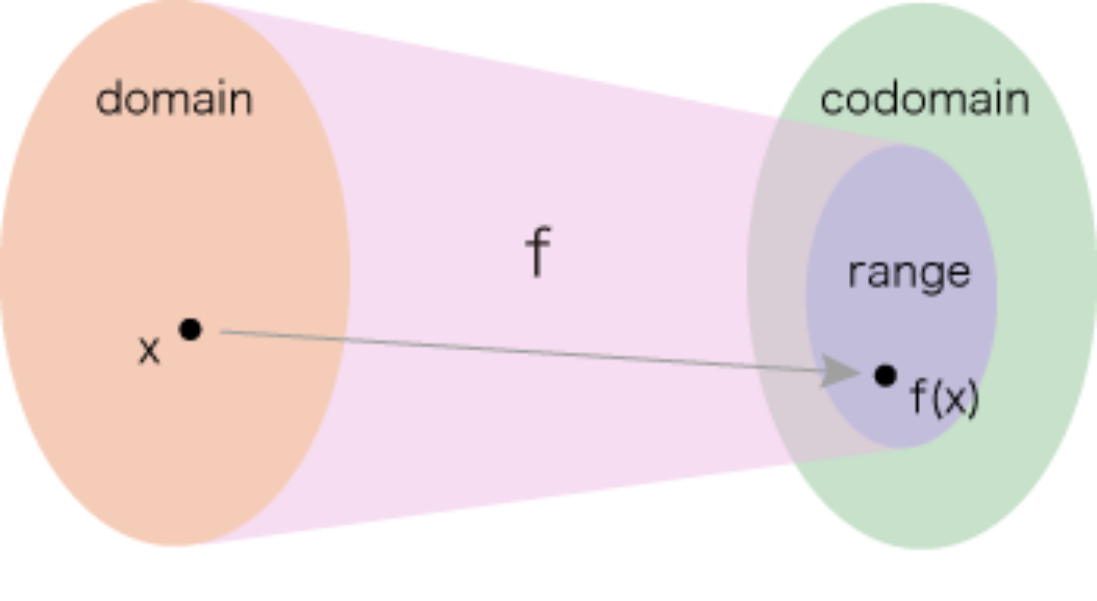
\includegraphics[width=\textwidth]{function_2.png}
% 			\end{center}
% 	\end{columns}
% \end{frame}

% \begin{frame}
% 	\frametitle{関数の一覧}
% 	% \begin{itemize}
% 		% \item 関数について、一覧表にしました。
% 		\begin{itemize}
% 			\item 代数関数までが中学校、
% 			\item 初等超越関数からが高校以降です。
% 		\end{itemize}
% 	% \end{itemize}
% 	\scriptsize
% 	\begin{center}
% 		% \caption{様々な関数}
% 		% \label{kansu}
% 		\begin{tabular}{|c|c|c|c|c|c|} \hline
% 			\multicolumn{5}{|c|}{関数} &	具体例 \\ \hline
% 			\color{red}
% 			\multirow{11}{*}{ \pbox<t>{初等関数} } & \multirow{6}{*}{ \pbox<t>{代数関数} } & \multirow{5}{*}{ \pbox<t>{有理関数} } & \multirow{4}{*}{ \pbox<t>{多項式関数} }	&	定数関数	& $f(x) = a$	\\ \cline{5-6}
% 			&&&& 一次関数	& $f(x) = ax + b$	\\ \cline{5-6}
% 			&&&& 二次関数	& $f(x) = ax^2 + bx + c$ \\ \cline{5-6}
% 			&&&& 三次関数	& $f(x) = ax^3 + bx^2 + cx + d$	\\ \cline{4-6}
% 			&&& \multicolumn{2}{c|}{分数関数}	& $f(x) = \dfrac{a}{x}$	\\ \cline{3-6}
% 			&& \multicolumn{3}{c|}{無理関数}	& $f(x) = \sqrt{x}$	\\ \cline{2-6}
% 			& \multirow{5}{*}{ \pbox<t>{初等超越関数} } & \multicolumn{3}{c|}{指数関数}	& $f(x) = e^x$	\\ \cline{3-6}
% 			&& \multicolumn{3}{c|}{対数関数}	& $f(x) = \ln (x)$	\\ \cline{3-6}
% 			&& \multicolumn{3}{c|}{三角関数}	& $f(x) = \sin x$	\\ \cline{3-6}
% 			&& \multicolumn{3}{c|}{双曲線関数}	& $f(x) = \sinh x$	\\ \cline{3-6}
% 			&& \multicolumn{3}{c|}{冪関数}	& $f(x) = x^a$	\\ \hline
% 			% \color{black}
% 			% \multirow{4}{*}{ \pbox<t>{特殊関数} } & \multicolumn{4}{c|}{ガンマ関数}	& $\Gamma (x)$	\\ \cline{2-6}
% 			% & \multicolumn{4}{c|}{ベータ関数}	& B$(x,y)$	\\ \cline{2-6}
% 			% & \multicolumn{4}{c|}{誤差関数}	& $erf(x)$	\\ \cline{2-6}
% 			% & \multicolumn{4}{c|}{デルタ関数}	& $\Delta$	\\ \hline
% 		\end{tabular}
% 	\end{center}
% \end{frame}

\begin{frame}
	\frametitle{関数とグラフ}
	\begin{block}{グラフとは}
		\begin{itemize}
			\item \alert{入力と出力との関係を平面図}に示しすことで、
			\item 視覚的に入力と出力との関係を理解しやすくしたもの
			% \item 具体的には、
			\begin{itemize}
				\item 入力 $x$ に対応して決まる出力の点を平面上に書き込む
				\item それを連続的に（直線または曲線で）つないだもの
			\end{itemize}
		\end{itemize}
	\end{block}

	\vspace{-5mm}
	\centering
	\begin{minipage}{.7\textwidth}
		\begin{columns}[c, onlytextwidth]
		\column{.4\linewidth}
			\begin{block}{関数を表すグラフ}
				\begin{itemize}
				\item 横軸は入力
				\item 縦軸が出力
				\item 赤い曲線は関数の軌跡
			\end{itemize}
			\end{block}
		\column{.58\linewidth}
			\begin{center}
			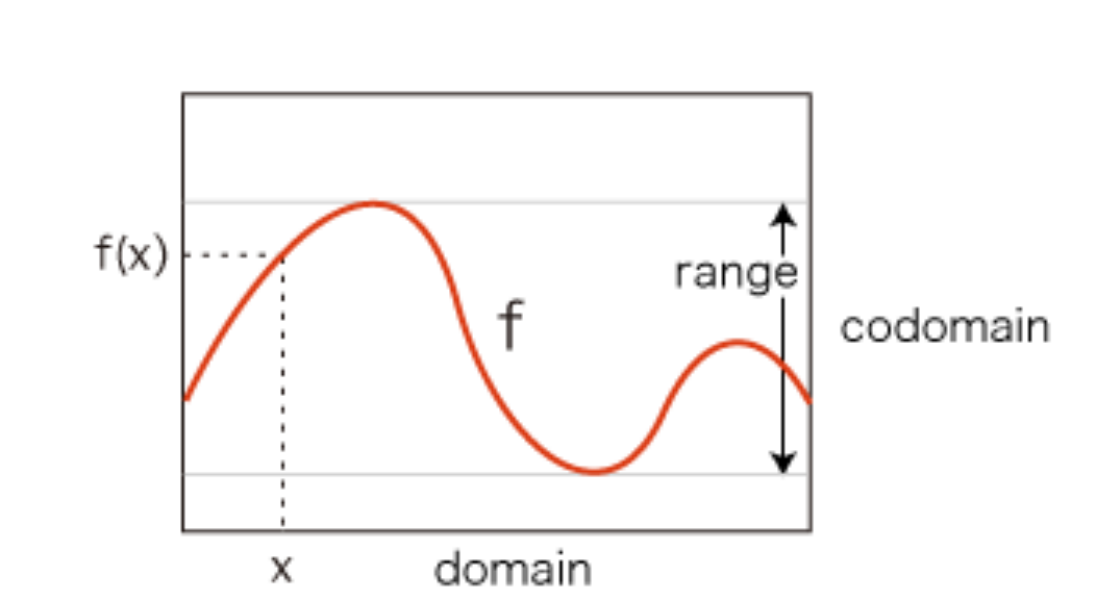
\includegraphics[width=\textwidth]{function_3.png}
			\end{center}
	\end{columns}
	\end{minipage}
\end{frame}
	
% \section{線型という意味を理解しよう}
\begin{frame}
	\frametitle{線型性とは}
	\begin{block}{線型という言葉を直感的にイメージ}
		\begin{itemize}
			\item \alert{「グラフに表した時に原点を通る直線となる性質」}
		\end{itemize}
	\end{block}
	
	\begin{block}{数学的な線型性の定義}
			\begin{itemize}
				\item 演算（写像）$f$ が、以下に示した2つの性質を満たすとき
				\begin{itemize}
					\item 加法性：任意の $x,y$ に対して
					\begin{equation*}
						f(x+y)=f(x)+f(y)
					\end{equation*}
					% \begin{align*}
					% 	f(x+y)=f(x)+f(y)
					% \end{align*}
					\item 斉次性：任意の $x,a$ に対して
					\begin{equation*}
						f(ax)=af(x)
					\end{equation*}
					% \begin{align*}
					% 	f(ax)=af(x)
					% \end{align*}
				\end{itemize}
			\end{itemize}
	\end{block}
\end{frame}

\begin{frame}
	\frametitle{線型性とは}
		\begin{itemize}
			\item 線型性を示す関数はたくさんあります。
			\begin{itemize}
				\item 以下の一次方程式が代表的
				\begin{equation*}
					y=ax
				\end{equation*}
				\item 比例の関係：入力の大きさが二倍 $\Leftrightarrow$ 出力も二倍
			\end{itemize}
			\item 加法性を利用し、小学校の応用問題としての旅人算も
		\end{itemize}
		\begin{itembox}[l]{旅人算の例}
			「A君とB君が 3km 離れた地点から向かい合って同時に出発しました。
		A君は毎分 30m、B君は毎分 70m で歩いたとすると、二人が出会うのは出発してから何分後ですか。」
		というような問題です。
		\end{itembox}
	% \begin{block}{旅人算の例}
	% 	「A君とB君が 3km 離れた地点から向かい合って同時に出発しました。
	% 	A君は毎分 30m、B君は毎分 70m で歩いたとすると、二人が出会うのは出発してから何分後ですか。」
	% 	というような問題です。
	% \end{block}
\end{frame}

\begin{frame}
	\frametitle{線型性の意味}
		% 小学校レベルの簡単な問題を考えてみましょう。
		\begin{itemize}
			\item 浴槽に水を溜めます。5分間流して100Lの水が溜まりました。
			\begin{itemize}
				\item 「1 分間流したときには何L溜まっていた？」\\
				比例より、 $1 \text{分} \times 100 L /5 \text{分}= 20 L$ ⇔ \textcolor{red}{過去を推定}
				\item「10 分では何L溜まるでしょう？」⇔ \textcolor{red}{未来を予測}
			\end{itemize}
			\item A蛇口は1分間で20L、B蛇口は5分間で150Lの水を貯められる。
			\begin{itemize}
				\item 「両方の蛇口から同時だと10分間では何L？」
				\item \textcolor{red}{加法性と斉次性を利用}すれば簡単に解ける
			\end{itemize}
		\end{itemize}
		\centering
		\begin{minipage}{.7\textwidth}
			\begin{itembox}[l]{線型性が成立する（と仮定する）ことで}
			\begin{itemize}
				\item 事象を重ね合わせながら
				\item 過去や未来の値を決定
			\end{itemize}
		\end{itembox}
		\end{minipage}
\end{frame}

% \section{物理的に考えましょう}
% \section{物理モデルと線型性}
\begin{frame}
	\frametitle{物理モデルについて}
	% \Large
	% 続いて、物理モデルとの関係で考えてみましょう。
	\begin{block}{物理モデルの考え方}
		\begin{itemize}
			\item モデルという言葉の意味は？
			\item \alert{「事象や理論の成り立ちを説明するための理解しやすい考え方」}
			\begin{itemize}
				\item 「地動説」を説明するために、「太陽系モデル」が提案
				\item 経済活動で利益の最大化に種々の「ビジネスモデル」
			\end{itemize}
			\item \alert{「モデルとは、対象とする事象を簡略化してその本質を表したもの」}
		\end{itemize}
	\end{block}

	\begin{block}{対象に応じて}
		\begin{itemize}
				\item 対象を物理現象にとったとき、「物理モデル」
				\item 定量的な解析のために数学を応用した「数理モデル」\\
				$\Rightarrow$ モデル化で使った概念を数式表現へ落とし込む
			\end{itemize}
	\end{block}
	% 我々の議論においては、レオロジーに関連する理論を説明するために使える考え方やイメージ図として物理モデルを利用して理解を深めていくわけです。
\end{frame}

\begin{frame}
	\frametitle{物理現象と線型応答}
        \begin{block}{我々の身の回りに起こっている実際の事柄}
            \begin{itemize}
                \item 非常に複雑な場合がほとんど
                \begin{itemize}
					\item 評価したい出力（応答）が分かりづらい
					\item 入力も不明確だったりする
				\end{itemize}
            \end{itemize}
        \end{block}
        \begin{alertblock}<2->{入力が小さい場合には}
            \begin{itemize}
                \item 応答が線型で取り扱える場合が多い
                \begin{itemize}
                    \item 加法性や斉次性が使える
                    \item 多種類の入力でもそれらが分割可能\\
                        \uncover<3->{\alert{分割できるということは独立に起きている事柄}}
                \end{itemize}
                \item<4> 事象の細かい部分を無視\alert{⇔単純化（近似）できるので理解が容易}
            \end{itemize}
        \end{alertblock}
\end{frame}

\begin{frame}
	\frametitle{物理モデルと線型性}
		\begin{itembox}[l]{簡単なまとめ}
			\begin{itemize}
				\item 実際の身の回りの現象
				\begin{itemize}
					\item \textcolor{blue}{非常に複雑}な場合がほとんど。
				\end{itemize}
				\item 線型現象であれば、取り扱いが容易。
				\begin{itemize}
					\item \textcolor{red}{微小な刺激に対しては、線形応答が期待}できる。
					\item 線形応答の重ね合わせで、\textcolor{red}{事象を近似}する価値は高い。
				\end{itemize}
				\item 線型性が成り立っているのであれば、
				\begin{itemize}
					\item 比例定数を調べることで、物質の性質を\textcolor{red}{容易に比較}できる
				\end{itemize}
			\end{itemize}
		\end{itembox}
		線型性を仮定できるような単純な物理モデルを利用して理解
\end{frame}

\begin{frame}
	\frametitle{まとめ}
	% この章では、物質の三態について物理化学的に考えてみました。
	\begin{boxnote}
		\vspace{-3mm}
		\begin{itemize}
			\item 関数について
			\begin{itemize}
				\item 関数とは入力と出力を関係づける方法
			\end{itemize} 
			\item 線形という意味
			\begin{itemize}
				\item グラフに表した時、原点を通る直線となる性質
				\item 加法性と斉次性を満たす
				\item 事象を重ね合わせながら過去や未来の値を決定
			\end{itemize} 
			\item 物理モデル？
			\begin{itemize}
				\item モデルとは事象を簡略化して本質を表したもの
				\item 線形性を利用して単純化（近似）して理解
			\end{itemize} 
		\end{itemize}
	\end{boxnote}
\end{frame}

\end{document}